\documentclass[journal,10pt,twocolumn]{article}
\usepackage{graphicx}
\usepackage[margin=0.5in]{geometry}
\usepackage[cmex10]{amsmath}
\usepackage{array}
\usepackage{booktabs}
\usepackage{mathtools}
\title{\textbf{Conic section Assignment}}
\author{Mohamed Hamdan}
\date{September 2022}


\providecommand{\norm}[1]{\left\lVert#1\right\rVert}
\providecommand{\abs}[1]{\left\vert#1\right\vert}
\let\vec\mathbf
\newcommand{\myvec}[1]{\ensuremath{\begin{pmatrix}#1\end{pmatrix}}}
\newcommand{\mydet}[1]{\ensuremath{\begin{vmatrix}#1\end{vmatrix}}}
\providecommand{\brak}[1]{\ensuremath{\left(#1\right)}}
\providecommand{\lbrak}[1]{\ensuremath{\left(#1\right.}}
\providecommand{\rbrak}[1]{\ensuremath{\left.#1\right)}}
\providecommand{\sbrak}[1]{\ensuremath{{}\left[#1\right]}}

\begin{document}

\maketitle
\paragraph{\textit{Problem Statement} - Find the area of the triangle formed by the lines joining the vertex of the parabola $x^2 = 12y$ to the ends of its latus rectum}

\section*{\large Solution}

\begin{figure}[h]
\centering
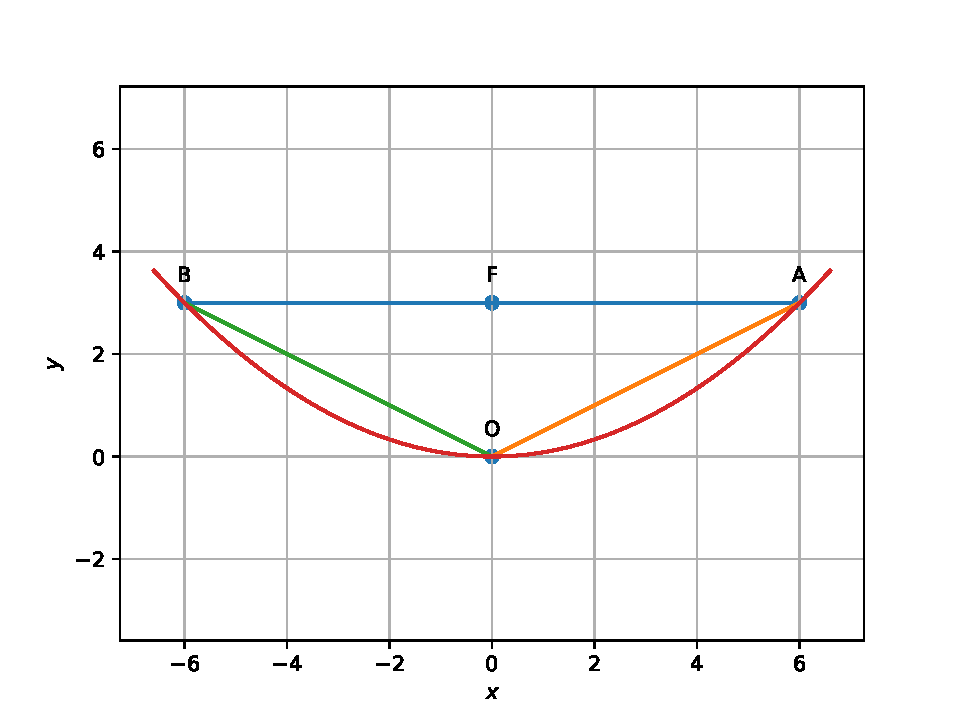
\includegraphics[width=1\columnwidth]{figs/fig1.pdf}
\caption{Triangle formed by vertex and ends of latus rectum of parabola $x^2 = 12y$}
\label{fig:parabola}
\end{figure}

The given equation of parabola $x^2 = 12y$ can be written in the general quadratic form as
\begin{align}
    \label{eq:conic_quad_form}
    \vec{x}^{\top}\vec{V}\vec{x}+2\vec{u}^{\top}\vec{x}+f=0
    \end{align}
where
\begin{align}
	\label{eq:V_matrix}
	\vec{V} &= \myvec{1 & 0\\0 & 0},
	\\
	\label{eq:u_vector}
	\vec{u} &= \myvec{0\\-6},
	\\
	\label{eq:f_value}
	f &= 0
	%\\
\end{align}

The parabola in (\ref{eq:conic_quad_form}) can be expressed in standard form (center/vertex at origin, major-axis - $x$ axis) as
\begin{align}
	\label{eq:conic_simp_parab}
	\vec{y}^{\top}\vec{D}\vec{y} &=  -2\eta\vec{e}_1^{\top}\vec{y}   & \abs{V} &= 0
	\end{align}
 where
\begin{align}
	\label{eq:conic_affine}
	\vec{x} = \vec{P}\vec{y}+\vec{c} \quad \text{(Affine Transformation)}
\end{align}
\begin{align}
	\label{eq:conic_parmas_eig_def}
	\vec{P}^{\top}\vec{V}\vec{P} &= \vec{D}. \quad \text{(Eigenvalue Decomposition)}
	\\
	\label{eq:eigevalV}
	\vec{D} &= \myvec{\lambda_1 & 0\\ 0 & \lambda_2}, 
	\\
	\vec{P} &= \myvec{\vec{p}_1 & \vec{p}_2}, \quad \vec{P}^{\top}=\vec{P}^{-1},
	\label{eq:eigevecP}
	\\
	\label{eq:eta}
	\eta &=\vec{u}^{\top}\vec{p}_1
	\\
	\vec{e}_1 &=\myvec{1 \\ 0}
	\end{align}

To find $\vec{c}$ which is the center of the parabola in (\ref{eq:conic_quad_form}), substitute (\ref{eq:conic_affine}) in (\ref{eq:conic_quad_form})
\begin{multline}
\brak{\vec{P}\vec{y}+\vec{c}}^T\vec{V}\brak{\vec{P}\vec{y}+\vec{c}}+2\vec{u}^T\brak{\vec{P}\vec{y}+\vec{c}} + f = 0, 
\end{multline}
yielding 
\begin{multline}
\vec{y}^T\vec{P}^T\vec{V}\vec{P}\vec{y}+2\brak{\vec{V}\vec{c}+\vec{u}}^T\vec{P}\vec{y} +  \vec{c}^T\vec{V}\vec{c} 
\\
+2\vec{u}^T\vec{c} + f= 0
\label{eq:conic_simp_one}
\end{multline}
%
From \eqref{eq:conic_simp_one} and \eqref{eq:conic_parmas_eig_def},
\begin{multline}
\vec{y}^T\vec{D}\vec{y}+2\brak{\vec{V}\vec{c}+\vec{u}}^T\vec{P}\vec{y} +  \vec{c}^T\brak{\vec{V}\vec{c} + \vec{u}}
\\
+ \vec{u}^T\vec{c} + f= 0
\label{eq:conic_simp}
\end{multline}
For a parabola $\abs{\vec{V}} = 0, \lambda_1 = 0$ and
\begin{align}
\vec{V}\vec{p}_1 = 0, 
\vec{V}\vec{p}_2 = \lambda_2\vec{p}_2.
\label{eq:conic_parab_eig_prop} 
\end{align}
where $\vec{p}_1,\vec{p}_2$ are the eigenvectors of $\vec{V}$ such that  \eqref{eq:conic_parmas_eig_def}
%
\begin{align}
\vec{P} = \myvec{\vec{p}_1 & \vec{p}_2},
\label{eq:eig_matrix}
\end{align}
Substituting \eqref{eq:eig_matrix}
in \eqref{eq:conic_simp},
\begin{multline}
	\vec{y}^T\vec{D}\vec{y}+2\brak{\vec{c}^T\vec{V}+\vec{u}^T}\myvec{\vec{p}_1 & \vec{p}_2}\vec{y}
\\
+  \vec{c}^T\brak{\vec{V}\vec{c} + \vec{u}}+ \vec{u}^T\vec{c} + f= 0
\\
\implies \vec{y}^T\vec{D}\vec{y}
\\
+2\myvec{\brak{\vec{c}^T\vec{V}+\vec{u}^T}\vec{p}_1  \brak{\vec{c}^T\vec{V}+\vec{u}^T}\vec{p}_2}\vec{y}
\\
+  \vec{c}^T\brak{\vec{V}\vec{c} + \vec{u}}+ \vec{u}^T\vec{c} + f= 0
\\
\implies \vec{y}^T\vec{D}\vec{y}
\\
+2\myvec{\vec{u}^T\vec{p}_1 & \brak{\lambda_2\vec{c}^T+\vec{u}^T}\vec{p}_2}\vec{y}
\\
+  \vec{c}^T\brak{\vec{V}\vec{c} + \vec{u}}+ \vec{u}^T\vec{c} + f= 0
\text{ from } \eqref{eq:conic_parab_eig_prop}     \nonumber \\
\\
\implies \lambda_2y_2^2+2\brak{\vec{u}^T\vec{p}_1}y_1+  2y_2\brak{\lambda_2\vec{c}+\vec{u}}^T\vec{p}_2
\\
+  \vec{c}^T\brak{\vec{V}\vec{c} + \vec{u}}+ \vec{u}^T\vec{c} + f= 0
\label{eq:conic_parab_foc_len_temp} 
\end{multline}
which is the equation of a parabola. 
Thus, \eqref{eq:conic_parab_foc_len_temp} 
can be expressed as \eqref{eq:conic_simp_parab} by choosing
\begin{align}
%\label{eq:eta}
\eta = \vec{u}^T\vec{p}_1
\end{align}
and $\vec{c}$ in \eqref{eq:conic_simp} such that
\begin{align}
\label{eq:conic_parab_one}
\vec{P}^{T}\brak{\vec{V}\vec{c}+\vec{u}} &= \eta\myvec{1\\0}
\\
\vec{c}^T\brak{\vec{V}\vec{c} + \vec{u}}+ \vec{u}^T\vec{c} + f&= 0
\label{eq:conic_parab_two}
\end{align}
Multiplying \eqref{eq:conic_parab_one} by $\vec{P}$ yields
\begin{align}
\label{eq:conic_parab_one_eig}
\brak{\vec{V}\vec{c}+\vec{u}} &= \eta\vec{p}_1,
\end{align}
which, upon substituting in \eqref{eq:conic_parab_two}
results in 
\begin{align}
\eta\vec{c}^T\vec{p}_1 + \vec{u}^T\vec{c} + f&= 0
\label{eq:conic_parab_two_eig}
\end{align}
\eqref{eq:conic_parab_one_eig} and \eqref{eq:conic_parab_two_eig} can be clubbed together to obtain \eqref{eq:conic_parab_c}.
\begin{align}
    \myvec{ \vec{u}^{\top}+\eta\vec{p}_1^{\top} \\ \vec{V}}\vec{c} &= \myvec{-f \\ \eta\vec{p}_1-\vec{u}}  &\abs{V} &= 0
    \label{eq:conic_parab_c}
    \end{align}
Substituting appropriate values from \eqref{eq:V_matrix}, \eqref{eq:u_vector}, \eqref{eq:f_value}, \eqref{eq:eigevecP}, and \eqref{eq:eta} into \eqref{eq:conic_parab_c}, the below matrix equation is obtained
\begin{align}
	\label{eq:vertex_system}
	\myvec{0&-12\\1& 0\\0& 0}\vec{c} = \myvec{0 \\0 \\0}\\
\end{align}
The augmented matrix for \eqref{eq:vertex_system} can be expressed as
\begin{align}
	\label{eq:vertex_solv1}
	\myvec{0&-12&\vrule&0\\1&0&\vrule&0\\0&0&\vrule&0}\\ 	
	\label{eq:vertex_solv2}
	\xleftrightarrow[]{R_1 \leftrightarrow R_2}\myvec{1&0&\vrule&0\\0&-12&\vrule&0\\0&0&\vrule&0}\\
	\label{eq:vertex_solv3}
	\xleftrightarrow[]{-\frac{R_2}{12} \leftarrow R_2}\myvec{1&0&\vrule&0\\0&1&\vrule&0\\0&0&\vrule&0}\\
	\label{eq:vertex_solv4}
	\implies\vec{c} = \myvec{0\\0}
\end{align}

From \eqref{eq:V_matrix}
  \begin{multline}
    \vec{V}^{\top} \vec{V}=\brak{\norm{\vec{n}}^2\vec{I}-e^2\vec{n}\vec{n}^{\top}}^{\top}
	  \\
	  \brak{\norm{\vec{n}}^2\vec{I}-e^2\vec{n}\vec{n}^{\top}}
    \\
    \implies \vec{V}^{2} = \norm{\vec{n}}^4\vec{I}+e^4\vec{n}\vec{n}^{\top}\vec{n}\vec{n}^{\top}
	  \\
	  -2e^2\norm{\vec{n}}^2\vec{n}\vec{n}^{\top}
    \\
    = \norm{\vec{n}}^4\vec{I} + e^4\norm{\vec{n}}^2\vec{n}\vec{n}^{\top}
	%  \\
	  - 2e^2\norm{\vec{n}}^2\vec{n}\vec{n}^{\top}
    \\
    = \norm{\vec{n}}^4\vec{I} + e^2\brak{e^2 - 2}\norm{\vec{n}}^2\vec{n}\vec{n}^{\top}
    \\
    = \norm{\vec{n}}^4\vec{I} + \brak{e^2 - 2}\norm{\vec{n}}^2\brak{\norm{\vec{n}}^2\vec{I}- \vec{V}}
    \end{multline}
%    
which can be expressed as
\begin{align}
  \vec{V}^{2} + \brak{e^2 - 2}\norm{\vec{n}}^2\vec{V} - \brak{e^2 - 1}\norm{\vec{n}}^4\vec{I}=0
  \label{eq:conic_quad_form_e_cayley}
\end{align}
Using the Cayley-Hamilton theorem, \eqref{eq:conic_quad_form_e_cayley} results in the characteristic equation, 
\begin{align}
  \lambda^{2} - \brak{2-e^2}\norm{\vec{n}}^2\lambda + \brak{1-e^2 }\norm{\vec{n}}^4=0
\end{align}
which can be expressed as
\begin{multline}
\brak{\frac{\lambda}{\norm{\vec{n}}^2}}^2 - \brak{2-e^2 }\brak{\frac{\lambda}{\norm{\vec{n}}^2}} + \brak{1-e^2 } = 0
\end{multline}
\begin{align}
  \implies \frac{\lambda}{\norm{\vec{n}}^2} = 1-e^2, 1
  \\
  \text{or, }\lambda_2 = \norm{\vec{n}}^2, \lambda_1 = \brak{1-e^2}\lambda_2 
  \label{eq:conic_quad_form_lam_cayley}
\end{align}
From   \eqref{eq:conic_quad_form_lam_cayley}, the eccentricity of \eqref{eq:conic_quad_form} is given by 
\begin{align}
	e &= \sqrt{1-\frac{\lambda_1}{\lambda_2}} 
	\label{eq:conic_quad_form_e}.   
\end{align}
%
% By inspection, we find that 
% \begin{align}
%   \frac{\lambda}}{\norm{\vec{n}}^2} = 1
%   \label{eq:conic_quad_form_lam2_cayley}
% \end{align}
%satisfies \eqref{eq:conic_quad_form_lam_cayley}.
Multiplying both sides of    \eqref{eq:V_matrix} by $\vec{n}$,
\begin{align}
\vec{V} \vec{n}&=\norm{\vec{n}}^2\vec{n}-e^2\vec{n}\vec{n}^{\top}\vec{n} 
\\
&=\norm{\vec{n}}^2\brak{1-e^2}\vec{n} 
 \\
% &=\frac{\lambda_1}{\lambda_2}\norm{\vec{n}}^2\vec{n} 
% \end{align}
% upon substituting from \eqref{eq:conic_quad_form_e}  and simplifying.  From the above, it is obvious that $\vec{n}$ is an eigenvector
% of $\vec{V}$.  Choosing 
% \begin{align}
%   \lambda_2 = \norm{\vec{n}}^2,
%   \label{eq:eigevecn_lam2}
% \end{align}  
% we obtain 
% \begin{align}
  &=\lambda_1 \vec{n} 
  \label{eq:eigevecn}
\end{align}  
from \eqref{eq:conic_quad_form_lam_cayley}
Thus,  $\lambda_1$ is the corresponding eigenvalue for $\vec{n}$.  From       \eqref{eq:eigevecP},   \eqref{eq:conic_quad_form_lam_cayley} and \eqref{eq:eigevecn}, 
\begin{align}
   \vec{n}&= \norm{\vec{n}}\vec{p}_1  = \sqrt{\lambda_2}\vec{p}_1 
\end{align}  
From \eqref{eq:u_vector} and \eqref{eq:conic_quad_form_lam_cayley},
\begin{align}
%   \label{eq:conic_quad_form_v}
% \vec{V} &=\norm{\vec{n}}^2\vec{I}-e^2\vec{n}\vec{n}^{\top}, 
% \\
%\label{eq:conic_quad_form_u}
\label{eq:focus_coord}
\vec{F}  &= \frac{ce^2\vec{n}-\vec{u}}{\lambda_2}
 \\
 \implies \norm{\vec{F}}^2  &= \frac{\brak{ce^2\vec{n}-\vec{u}}^{\top}\brak{ce^2\vec{n}-\vec{u}}}{\lambda_2^2}
 \\
 \implies \lambda_2^2\norm{\vec{F}}^2  &= c^2e^4\lambda_2-2ce^2\vec{u}^{\top}\vec{n}+\norm{\vec{u}}^2
 \label{eq:conic_quad_form_u_temp}
% f &= \norm{\vec{n}}^2\norm{\vec{F}}^2-c^2e^2
% %\\
    \end{align}
    Also, \eqref{eq:f_value} can be expressed as
    \begin{align}
    \lambda_2\norm{\vec{F}}^2 &= f+c^2e^2
    \label{eq:conic_quad_form_f_temp}
\end{align}
From  \eqref{eq:conic_quad_form_u_temp} and     \eqref{eq:conic_quad_form_f_temp},
\begin{align}
c^2e^4\lambda_2-2ce^2\vec{u}^{\top}\vec{n}+\norm{\vec{u}}^2 = \lambda_2\brak{f+c^2e^2}
\end{align}
\begin{multline}
\implies \lambda_2e^2\brak{e^2-1}c^2-2ce^2\vec{u}^{\top}\vec{n}
	\\
	+\norm{\vec{u}}^2 - \lambda_2 f = 0
\end{multline}
yielding
\begin{align}
c &= 
  \begin{cases}
    \frac{e\vec{u}^{\top}\vec{n} \pm \sqrt{e^2\brak{\vec{u}^{\top}\vec{n}}^2-\lambda_2\brak{e^2-1}\brak{\norm{\vec{u}}^2 - \lambda_2 f}}}{\lambda_2e\brak{e^2-1}} & e \ne 1
    \\
    \frac{\norm{\vec{u}}^2 - \lambda_2 f   }{2e^2\vec{u}^{\top}\vec{n}} & e = 1
  \end{cases}
  \label{eq:conic_quad_form_F}.
\end{align}

The points of intersection of the line 
\begin{align}
	L: \quad \vec{x} = \vec{q} + \mu \vec{m} \quad \mu \in \mathbf{R}
\label{eq:conic_tangent}
\end{align}
with the conic section in \eqref{eq:conic_quad_form} are given by
\begin{align}
\vec{x}_i = \vec{q} + \mu_i \vec{m}
\label{eq:conic_tangent_pts}
\end{align}
%
where
{\tiny
\begin{multline}
\mu_i = \frac{1}
{
\vec{m}^T\vec{V}\vec{m}
}
\lbrak{-\vec{m}^T\brak{\vec{V}\vec{q}+\vec{u}}}
\\
\pm
\rbrak{\sqrt{
\sbrak{
\vec{m}^T\brak{\vec{V}\vec{q}+\vec{u}}
}^2
-
\brak
{
\vec{q}^T\vec{V}\vec{q} + 2\vec{u}^T\vec{q} +f
}
\brak{\vec{m}^T\vec{V}\vec{m}}
}
}
\label{eq:tangent_roots}
\end{multline}
}
\\
Substituting \eqref{eq:conic_tangent}
in \eqref{eq:conic_quad_form}, 
\begin{align}
\brak{\vec{q} + \mu \vec{m}}^T\vec{V}\brak{\vec{q} + \mu \vec{m}}  
\\
+ 2 \vec{u}^T\brak{\vec{q} + \mu \vec{m}}+f &= 0
\\
\implies \mu^2\vec{m}^T\vec{V}\vec{m} + 2 \mu\vec{m}^T\brak{\vec{V}\vec{q}+\vec{u}} 
\\
+ \vec{q}^T\vec{V}\vec{q} + 2\vec{u}^T\vec{q} +f &= 0
\label{eq:conic_intercept}
\end{align}
Solving the above quadratic in \eqref{eq:conic_intercept}
yields \eqref{eq:tangent_roots}.

The area of a triangle whose vertices are $\vec{A}, \vec{B}$ and $\vec{O}$ is given by
\begin{align}
	ar(AOB) = \frac{1}{2}\norm{(\vec{A-O})\times(\vec{B-O})}
	\label{eq:tri_area}
\end{align}

\section*{\large Construction}
The input parameters are $\vec{V}$ from \eqref{eq:V_matrix}, $\vec{u}$ from \eqref{eq:u_vector} and $f$ from \eqref{eq:f_value}\\\\
{
\setlength\extrarowheight{5pt}
\begin{tabular}{|c|c|c|}
	\hline
	\textbf{Symbol}&\textbf{Value}&\textbf{Description}\\
	\hline
	$\vec{P}$&\myvec{0&1\\1&0}&eigenvectors of $\vec{V}$\\[5pt]
	\hline
	$\vec{O}$&$\myvec{0\\0}$&center of parabola\\
	\hline
	$\eta$&$\vec{u}^{\top}\vec{p}_1 = -6$&from \eqref{eq:eta}\\[5pt]
	\hline
	$\lambda_2$&$\vec{e}_2^{\top}D\vec{e}_2 = 1$&from \eqref{eq:eigevalV}\\[5pt]
	\hline
	$\vec{n}$&$\sqrt{\lambda_2}\vec{p_1} = \myvec{0\\1}$&normal to directrix\\[5pt]
	\hline
	$c$&from \eqref{eq:conic_quad_form_F}&$\vec{n}^\top\vec{x} = c$\\
	\hline
	$\vec{F}$&$\myvec{0\\3}$&focus from \eqref{eq:focus_coord}\\[5pt]
	\hline
	$\vec{m}$&$\myvec{1\\0}$&latus rectum direction vector\\[5pt]
	\hline
	$\myvec{\vec{A} \\ \vec{B}}$&$\myvec{\vec{F} + \mu_1\vec{m} \\ \vec{F} + \mu_2\vec{m}}$&$\mu_1, \mu_2$ from \eqref{eq:tangent_roots}\\[5pt]
	\hline
	ar(AOB)&18 sq units&from \eqref{eq:tri_area}\\
	\hline
\end{tabular}
}

\end{document}
